
\section{Malloc routines}\label{sec:malloc}

Consider creating a producer-consumer program using PiP, where one PiP
task serves as the producer and another as the consumer. In contrast
to the traditional process approach, PiP does not require an IPC
(Inter Process Communication) system call. Passing pointers pointing
at data to be transmitted from the producer to the consumer is all
that is necessary.  

There is a problem here. If the given data was allocated by the
\linuxfunc{malloc} function, the consumer will \linuxfunc{free} the
passed data. As previously mentioned, each PiP task has a unique set
of \linuxfunc{malloc} and \linuxfunc{free} procedures connected to
static variables that hold and manage a memory pool. When it is no
longer required, the consumer tries to \linuxfunc{free} the data it
has obtained from the producer's memory pool. Unfortunately, 
because the consumer's \linuxfunc{free} procedure is unaware of the
memory space that the producer allocated, it fails
(Figure~\ref{fig:cross-malloc-free-issue}). I gave this circumstance
the moniker {\it cross-malloc-free}. 

\begin{figure}[ht]
\centering
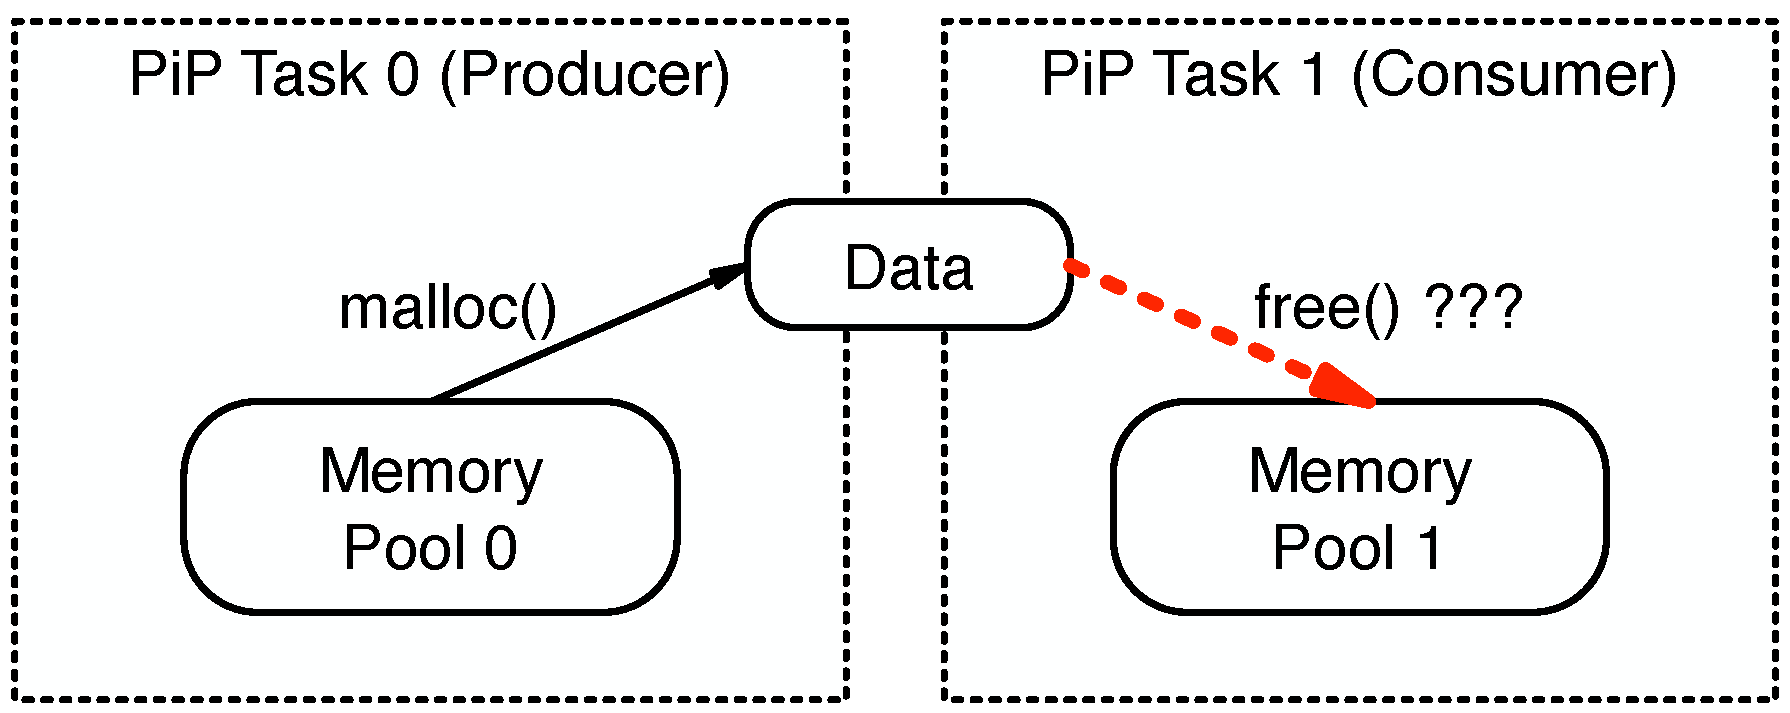
\includegraphics[width=0.7\columnwidth]{malloc/Figs/ProducerConsumer.pdf}
\caption{Cross-Malloc-Free Issue}
\label{fig:cross-malloc-free-issue}
\end{figure}

I gave it a shot using the {\tt malloc} functions that Glibc provides
and discovered that while it doesn't always work, it usually does. I'm
not sure why this works (again, {\it in most circumstances}) with the 
Glibc {\tt malloc} routines, but I believe it's important to avoid
this circumstance.

\begin{figure}[ht]
\centering
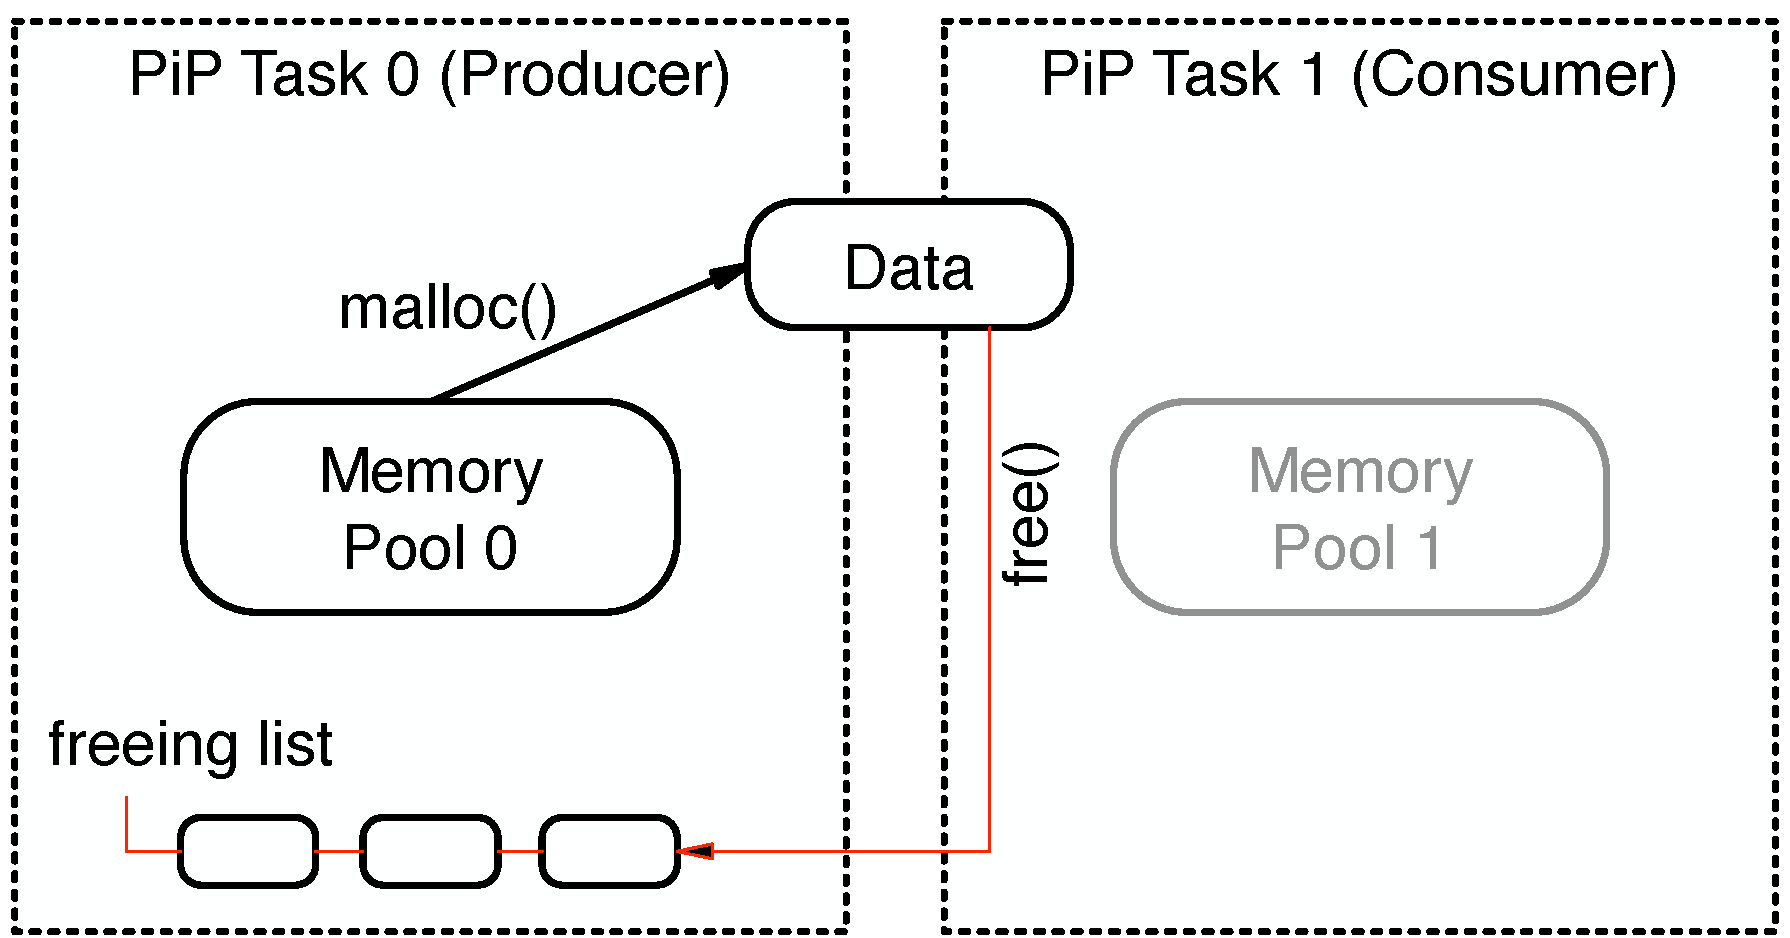
\includegraphics[width=0.7\columnwidth]{malloc/Figs/CrossMallocFree.pdf}
\caption{Cross-Malloc-Free with Freeing List}
\label{fig:cross-malloc-free}
\end{figure}

In order to address this, the PiP library wraps the {\tt malloc}
functions, as seen in Table 3.3. The \linuxfunc{malloc} wrapper
function embeds  the information about who allocated a memory
space. When this region is to be \linuxfunc{free}ed, the
\linuxfunc{free} wrapper function connects the region to the freeing 
list of the task allocating the region. When one of the wrapper
functions for {\tt malloc} is called, the regions in the freeing list
are really \linuxfunc{free}ed (Figure~\ref{fig:cross-malloc-free}). 
